\documentclass[11pt]{article}

\usepackage{graphicx}
\usepackage{fancyhdr}
\setlength{\topmargin}{-.5in}
\setlength{\textheight}{9in}
\setlength{\oddsidemargin}{.125in}
\setlength{\textwidth}{6.25in}
\graphicspath{images/}
\begin{document}
\title{Hacker News}
\author{Robert Game, Chris Johns, Tsz-Him Kwan, Richard Sommerville}
\date{Mobile Application Development}
\maketitle

\section*{Project Overview}
For this Group Coursework Team 11 have created an application to allow access from Android to the popular community-based news website Hacker News. Hacker News is a content website which is gaining popularity in the technical community, it is an aggregation of tech news, articles, discussions and job listings which is controlled by 'Karma', a score which is decided by the users on the website.  When deciding on our initial designs we found that other community websites had a strong presence on the Google Play Store and as such other applications such as Reddit Sync or Reddit is Fun have a strong user base. However, in comparison we could only find one other Hacker News application which had been created as a side project, and as such did not have full developer support. Our choice of Hacker News stemmed from this gap in the market.
\\
\\
The visual feel of this application has taken shape from the recent release of Google's Android 5.0 Lollipop and it's adoption of Material Design. Our initial concept drawings we created with these design guidelines in mind and the final build of our application has been checked against these in order to de clare our application as “Fully Material”. The adoption of Material Design is a current trend in the Play Store and there is a trend of users favouring applications for their adoption of the latest standards. This added two new designs for the application, one for pre-API 21 devices and one for API 21+ devices with Material support. The addition of Material Designs libraries gives the application an added polish on later devices whilst still maintaining a full user experience on 
\\
\\
The main activity of our application is the ‘Top 100' page. This page can include Stories, Polls, AskHN and Jobs ordered by their popularity on the website. With the recent release of the Lollipop API Google have also added the Recycler View and recommend it's use for display of large amounts of data in a list format we opted to use this in order to ensure that application is up to date with current standards. Our main page contains one fragment in the form of a Recycler View, a newer implementation of Android's Listview which is more efficient and less taxing on the device CPU as it requires  fewer ID lookups by storing references to UI elements in a ViewHolder, this means that objects need to only be inflated once when the ViewHolder is created. By default our application displays the first ten stories in the Top 100. Scrolling down from these will trigger a load of a further ten, this will continue until the Top 100 is displayed in it's entirety. Each item within the view displays information pertinent to the story it relates to. From this the User can launch the webview or comments relating to this story.
\\
\\
Connectivity to Hacker News is provided by Hacker News' own API implemented in Firebase. Firebase is an API provider which has been created with platform compatibility in mind, providing an easy-to-use API for smaller companies that cannot implement their own data solutions for real-time requests of data. Connecting to this API is done through the use of the Firebase API to make requests to Hacker News' API implemented in Firebase. Firebase then returns a JSON data object. Our back-end code uses this JSON object to examine the returned Threads and convert them into either a Story, Poll, AskHN or Job object. This is also the case for Items, working out whether the returned item is a Comment or a Poll Option.

\section*{Application Functionality}

\subsection*{Top 100 View}
\begin{center}
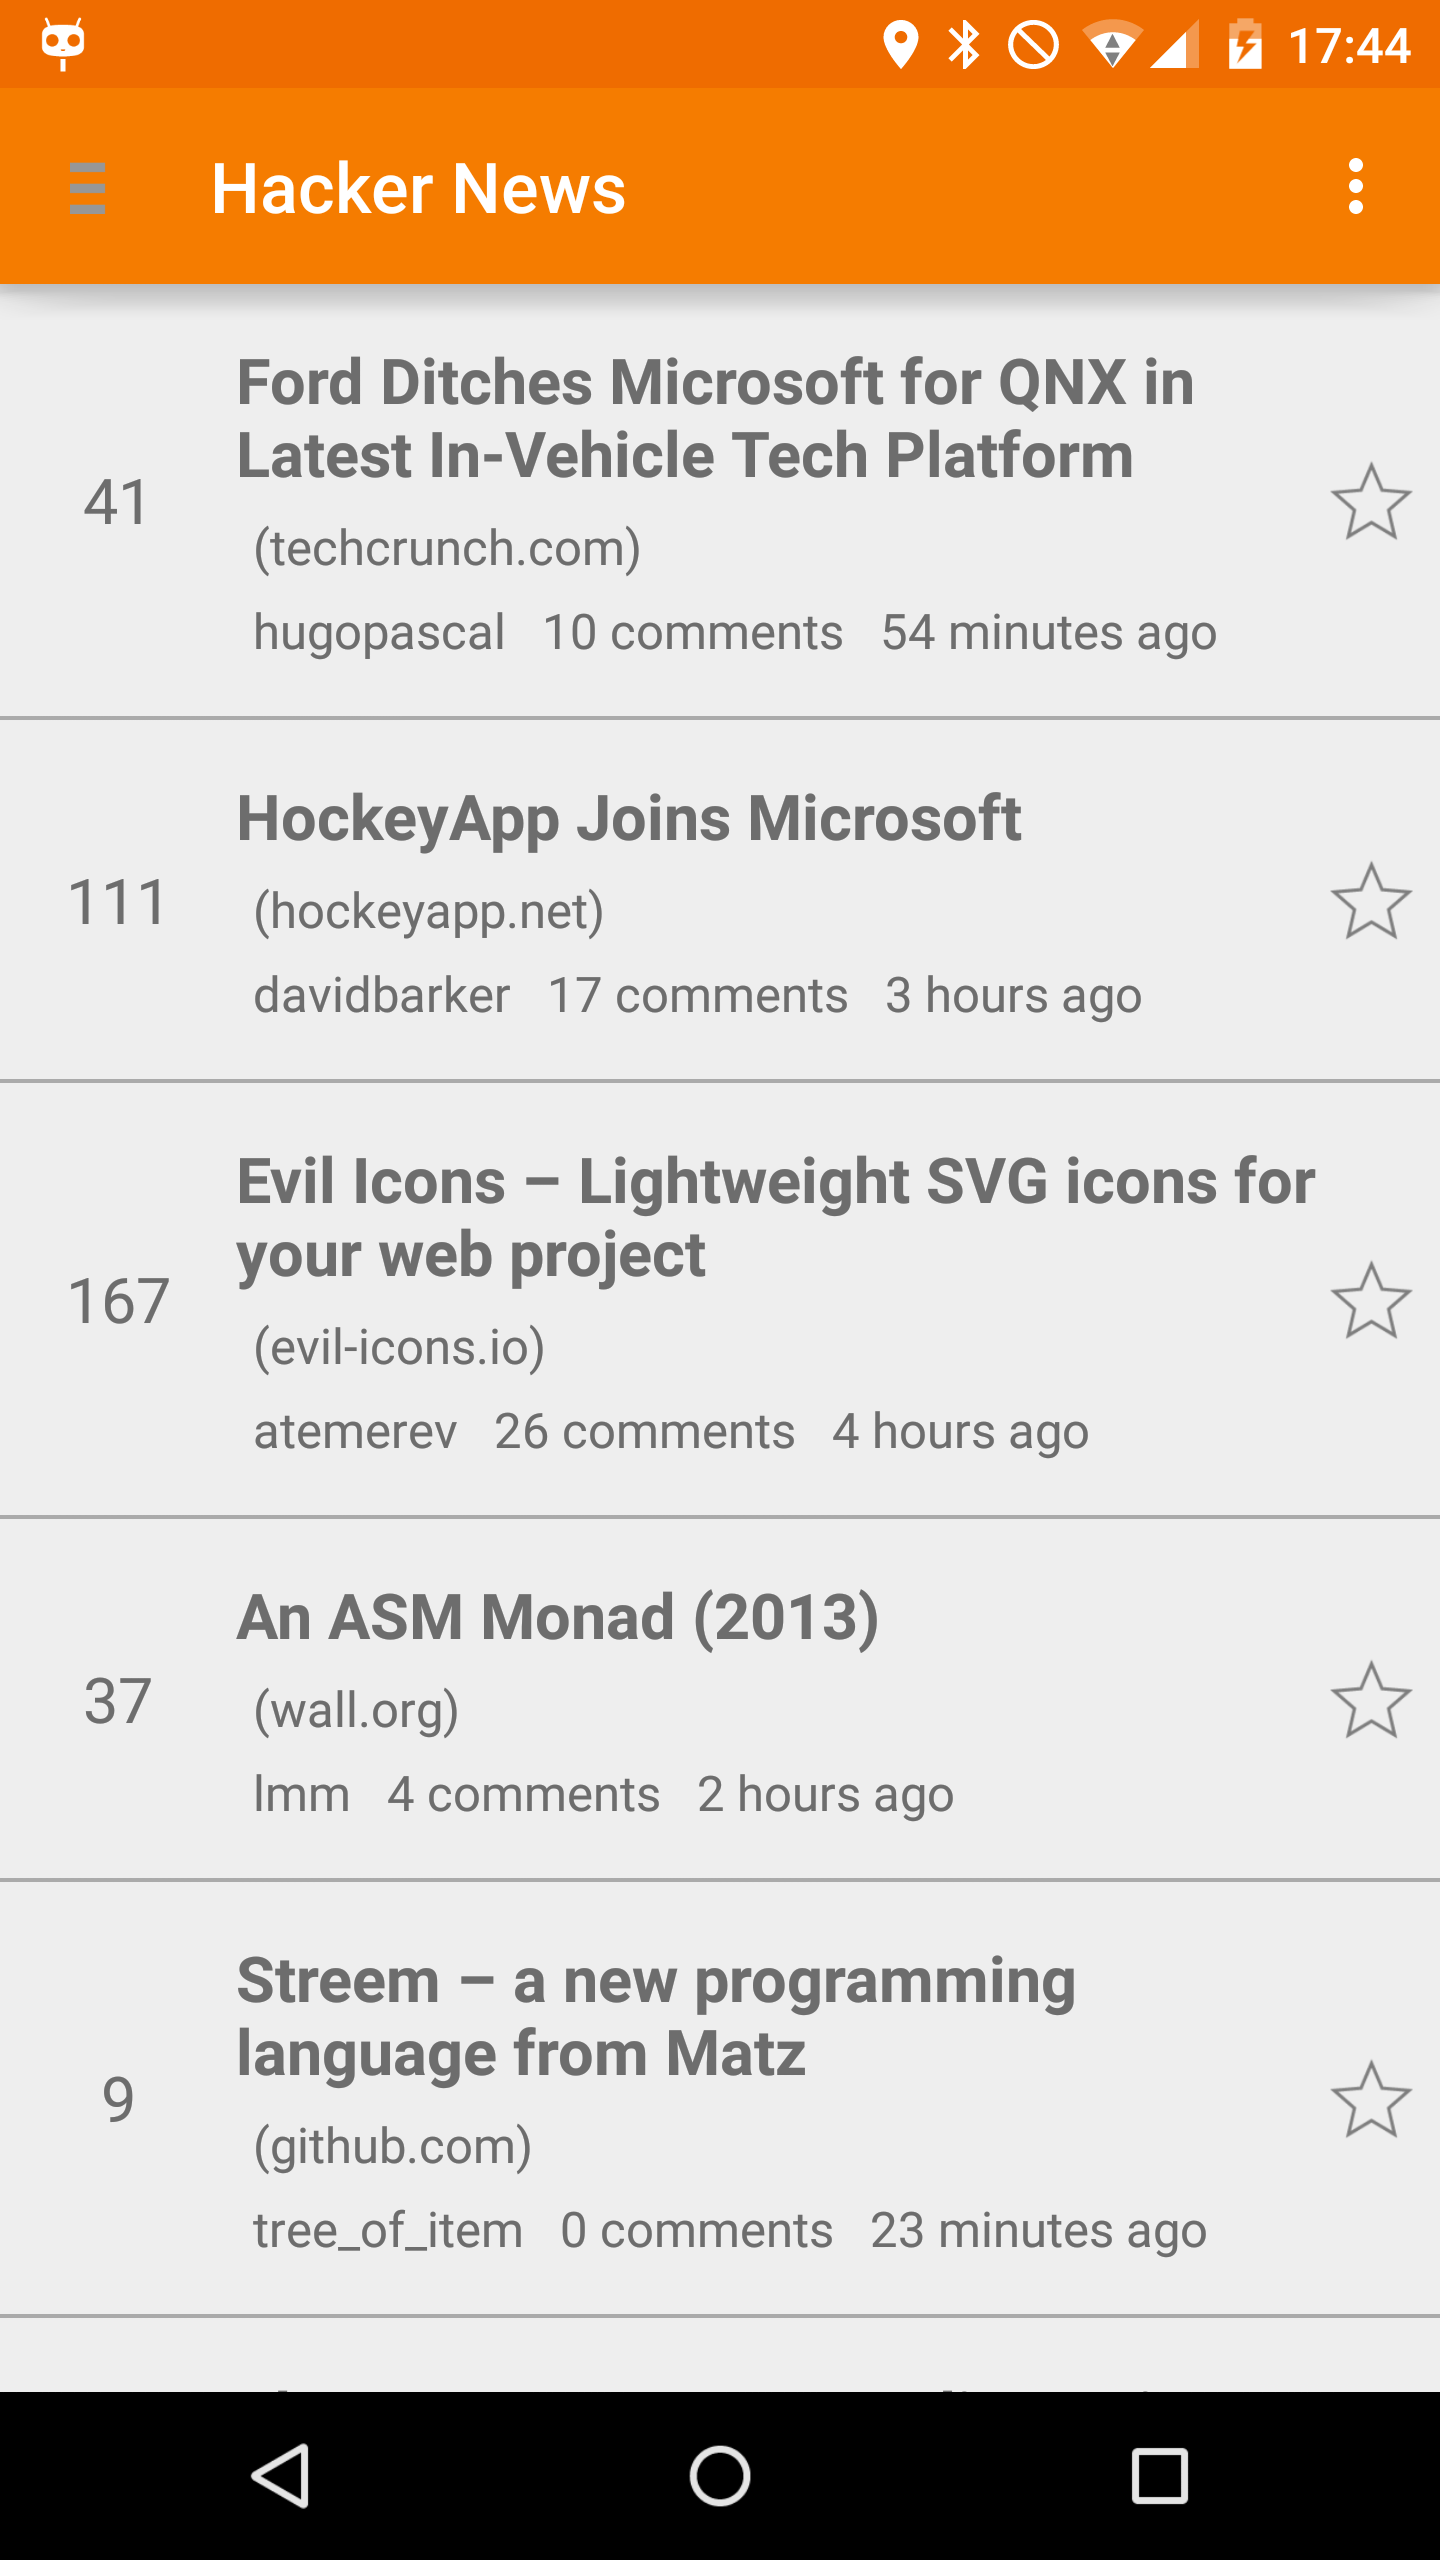
\includegraphics[width=0.3\textwidth]{threadView.png}
\end{center}

The Top 100 Stories are the displayed when the application is first opened. This view is a mirror of what is displayed on Hacker News at the current time. By default the first ten stories are displayed and further stories are fetched as the user scrolls down the view. This view displays each Thread along with it's relevant Title, Score, Domain, Submitter, Number of Comments and the Time since it was posted. The user can access a Story by tapping the Title, this will open a webview and load the relevant URL for the chosen story. Alternatively the user can tap the number of comments, this will open the comment view.
\\
\\
The top left ‘Burger' menu can be expanded to allow the user to choose between Threads and Users. The top right dots can be tapped to access the settings for the application. Hitting the Refresh button will initiate a new request to the Hacker News API and update the stories shown on the page.
\\
\\
Users can also use this screen to follow a particular thread. When pressing on the star icon on an item they will add this story to their Subscribed Stories. By doing this the application will store the id of a story to the devices local storage. The application will routinely check these stories for any new comments and will send the user updates via push notifications.
\\
\\
In addition to the above features the user can also tap and hold on an item, doing this will open any stories will open the relevant webpage in their applications web browser.

\subsection*{Comments View}

\begin{center}
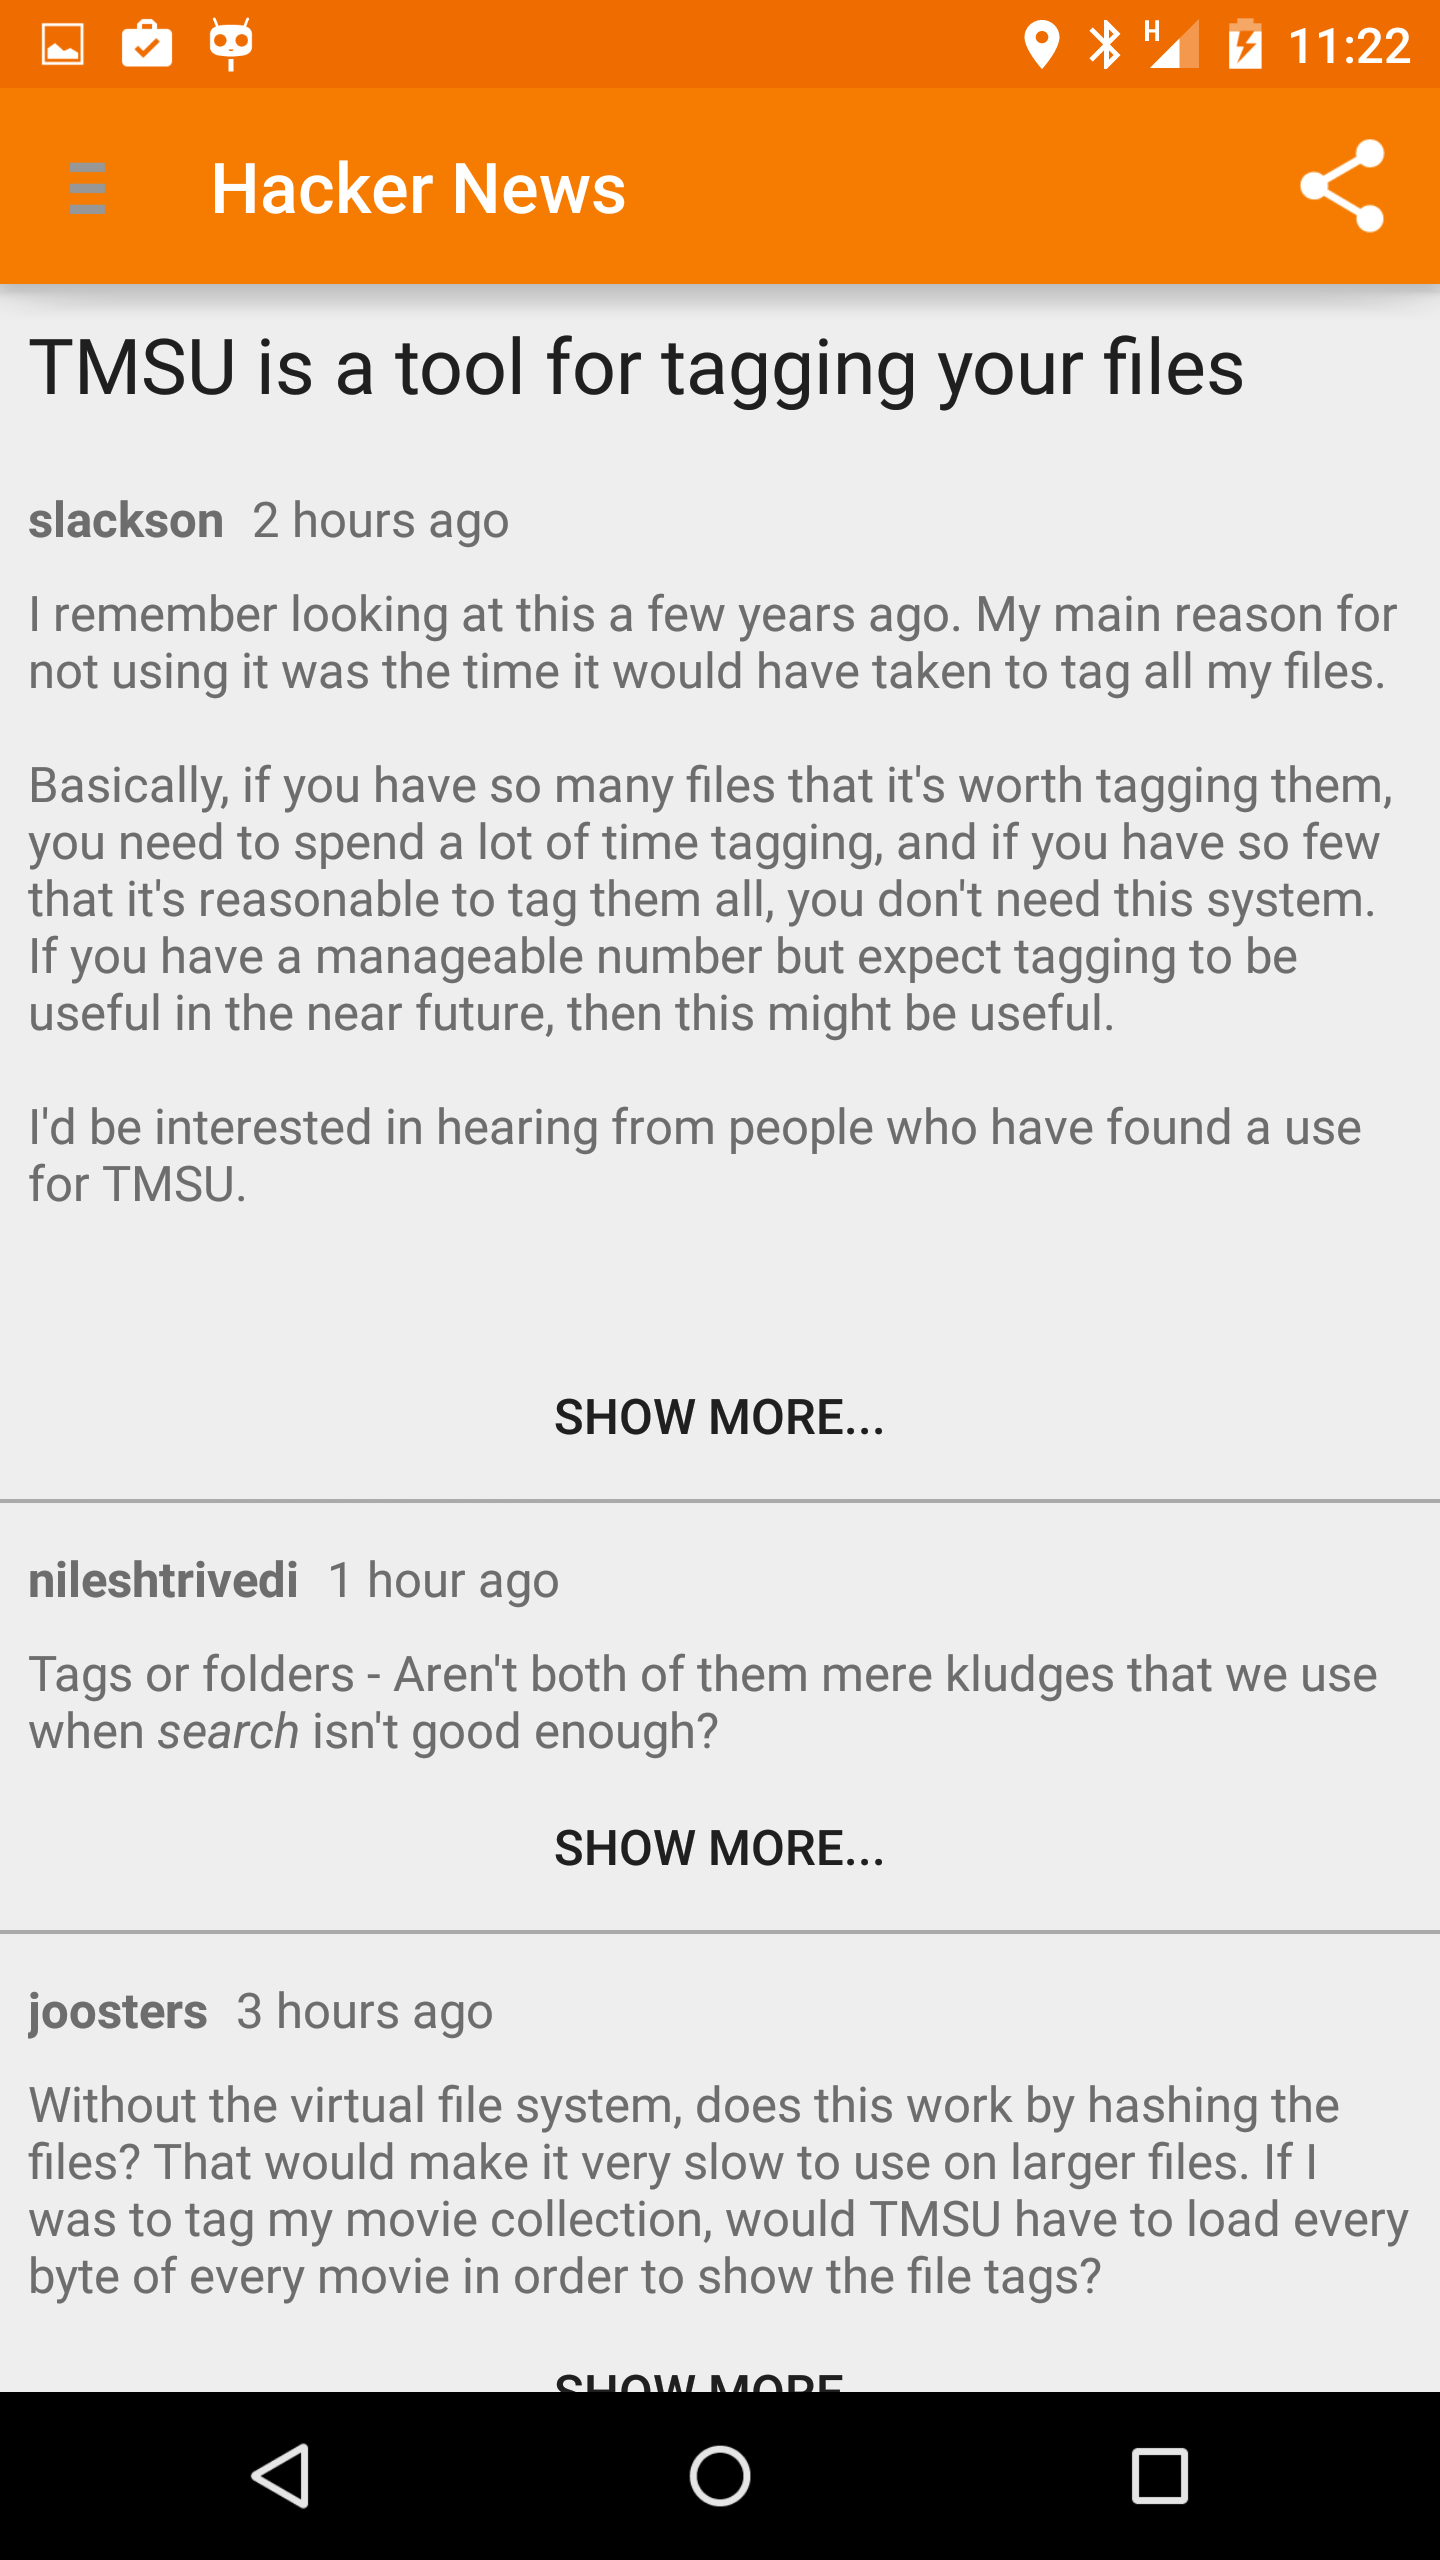
\includegraphics[width=0.3\textwidth]{comments.png}
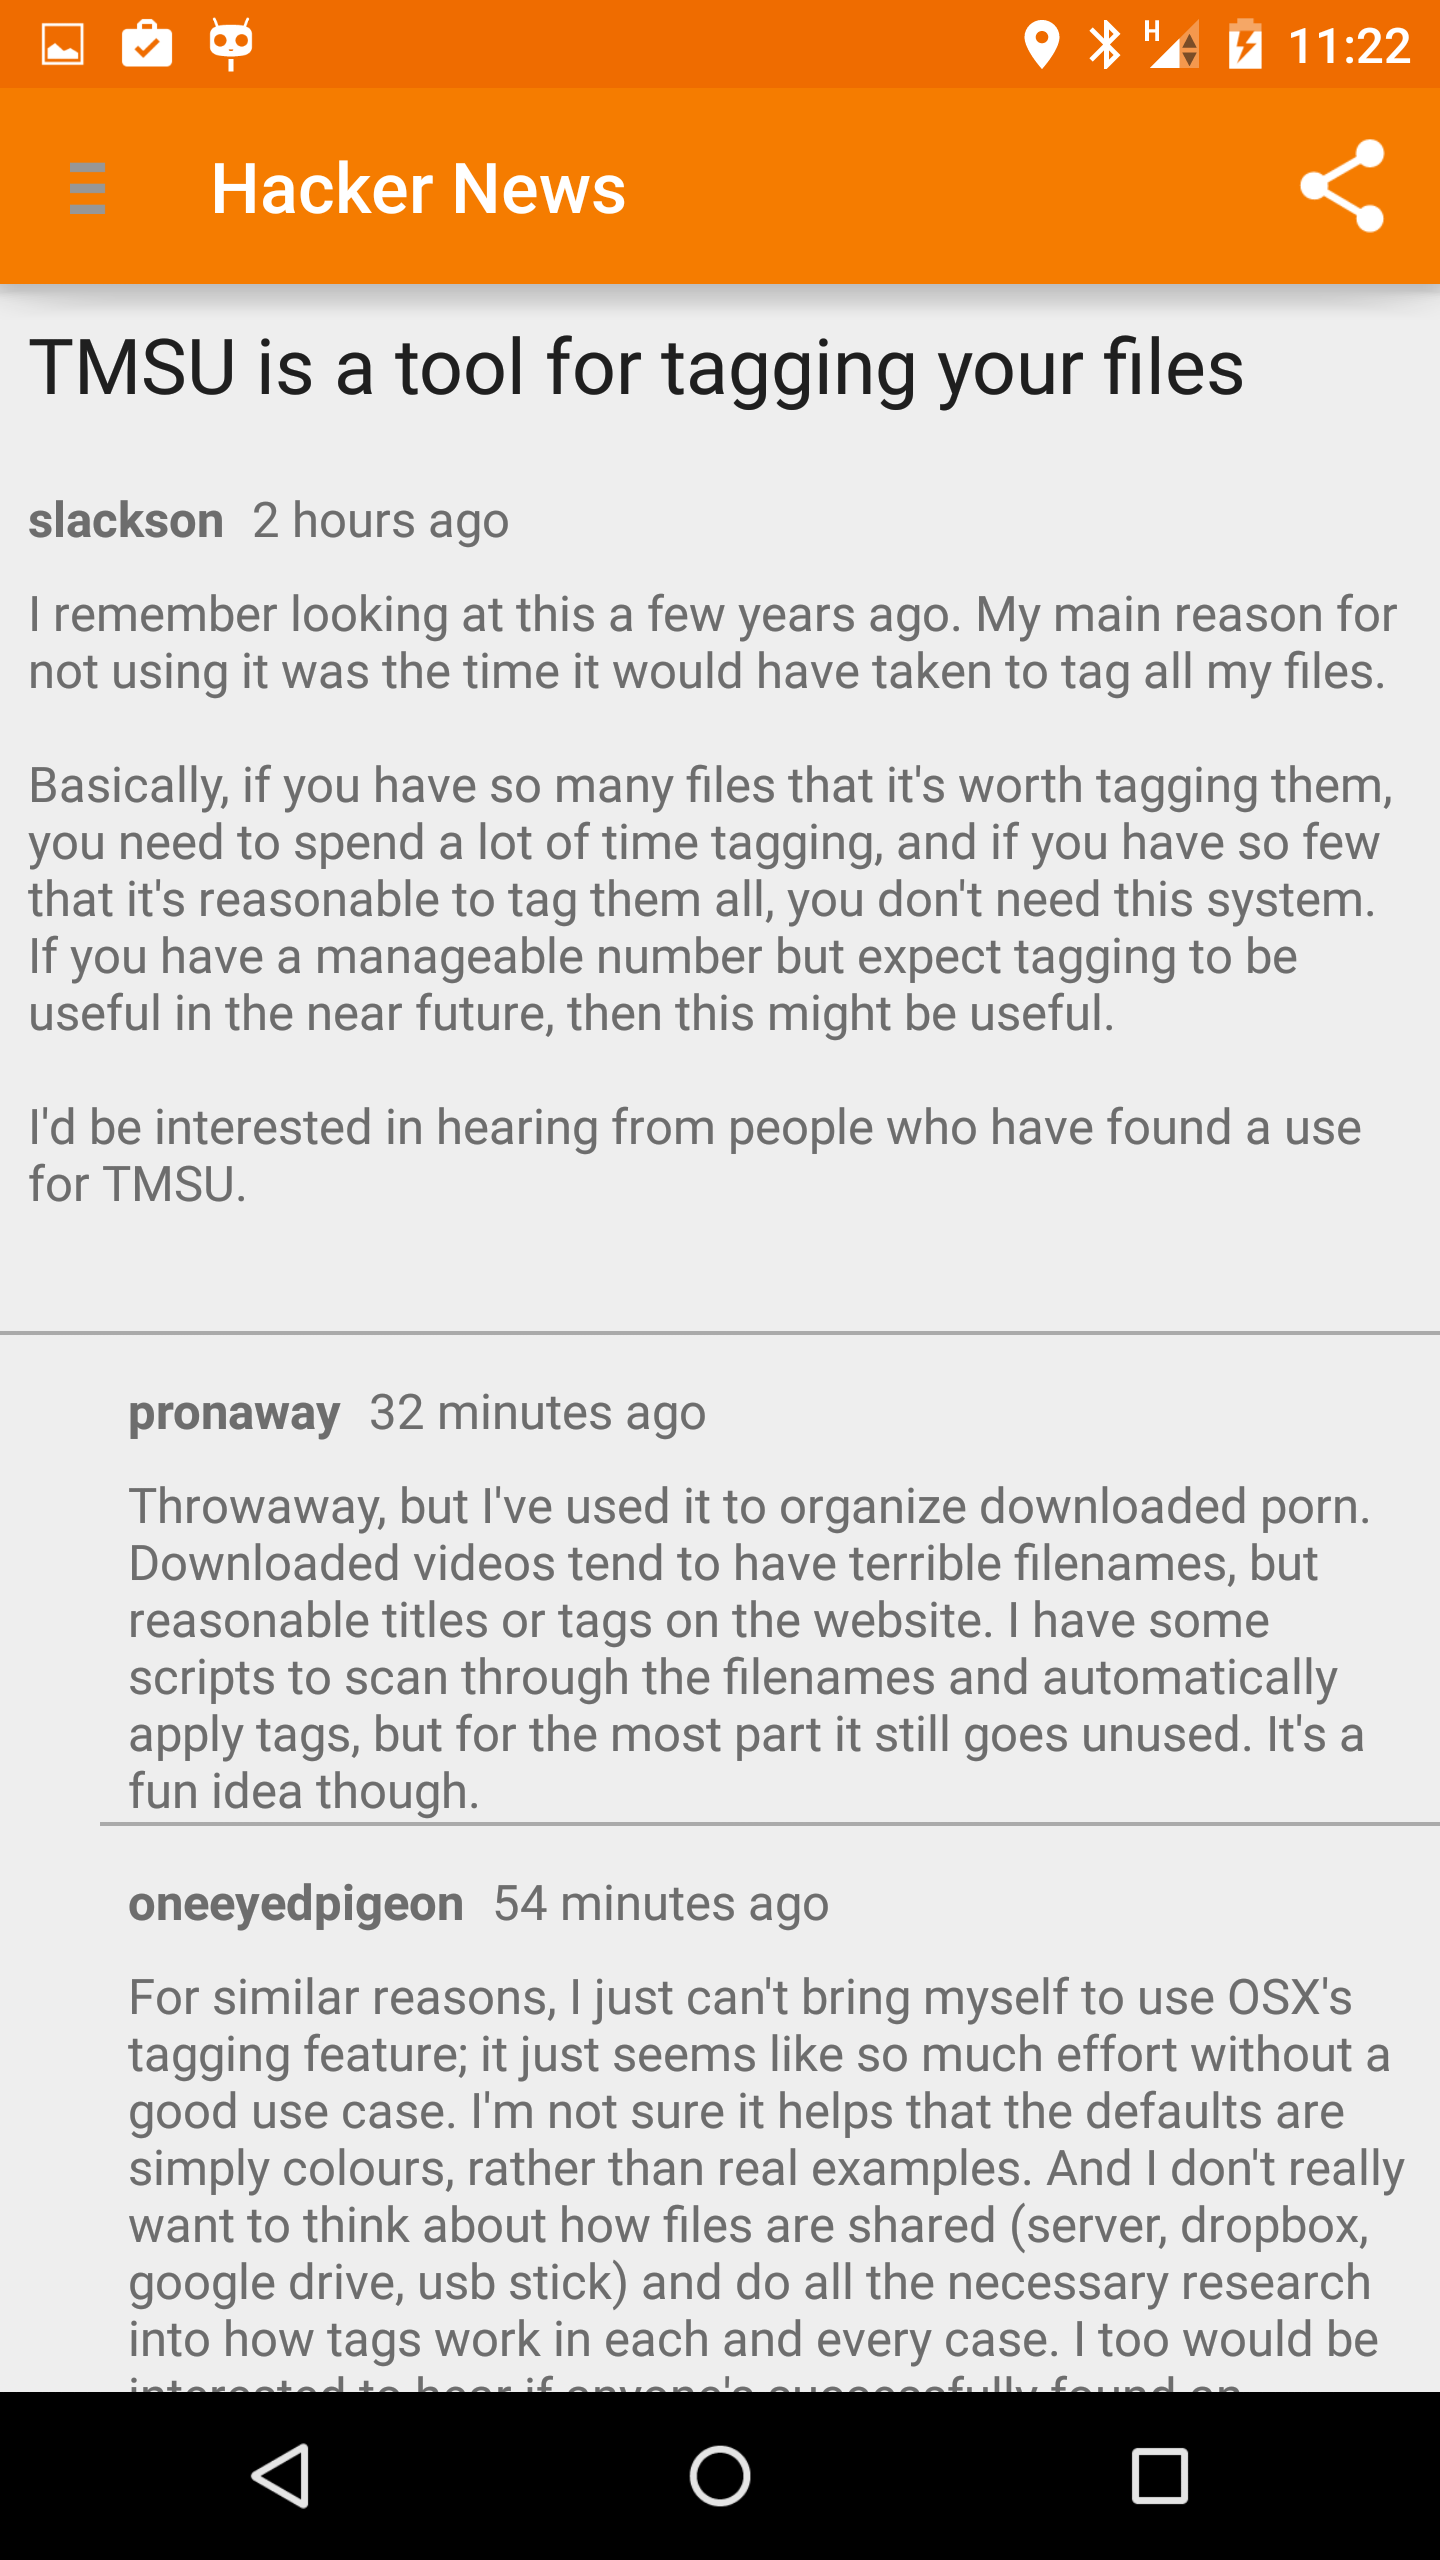
\includegraphics[width=0.3\textwidth]{commentsExpanded.png}
\end{center}

When a user taps the Comments on a given Thread the application will open the Comments View. Comments on Hacker News are given a tree structure where top-level comments can have children, these children can span multiple levels in the tree. On first load of this view only top-level comments are display, this was decided and agree on both a technical and UX standpoint as first because top-level comments are more relevant to a user at a quick glance, ensuring that they do not need to scroll in order to see all comments. Secondly because of each comment is defined as an Item within the API. In order to fetch second-layer comments for a post an API call is required based on it's parents id. If this needed to be done the load added to both the CPU and Network requests would increase significantly. To avoid this we have added a “Show More” button at the base of each comment. If a user intends to see the next level of comments they can press this to display them. Comments are indented according to their layer in the hierarchy. This is shown above.
\\
\\
In addition to the comment functionality, a user can also share their current location in the app using other applications on their device. For example the Share functionality in the screenshots above are set to share to Hangouts should the user press on that icon, if another application is desired pressing the share icon will display a list of relevant applications defined by Android. 

\subsection*{Web View}

\begin{center}
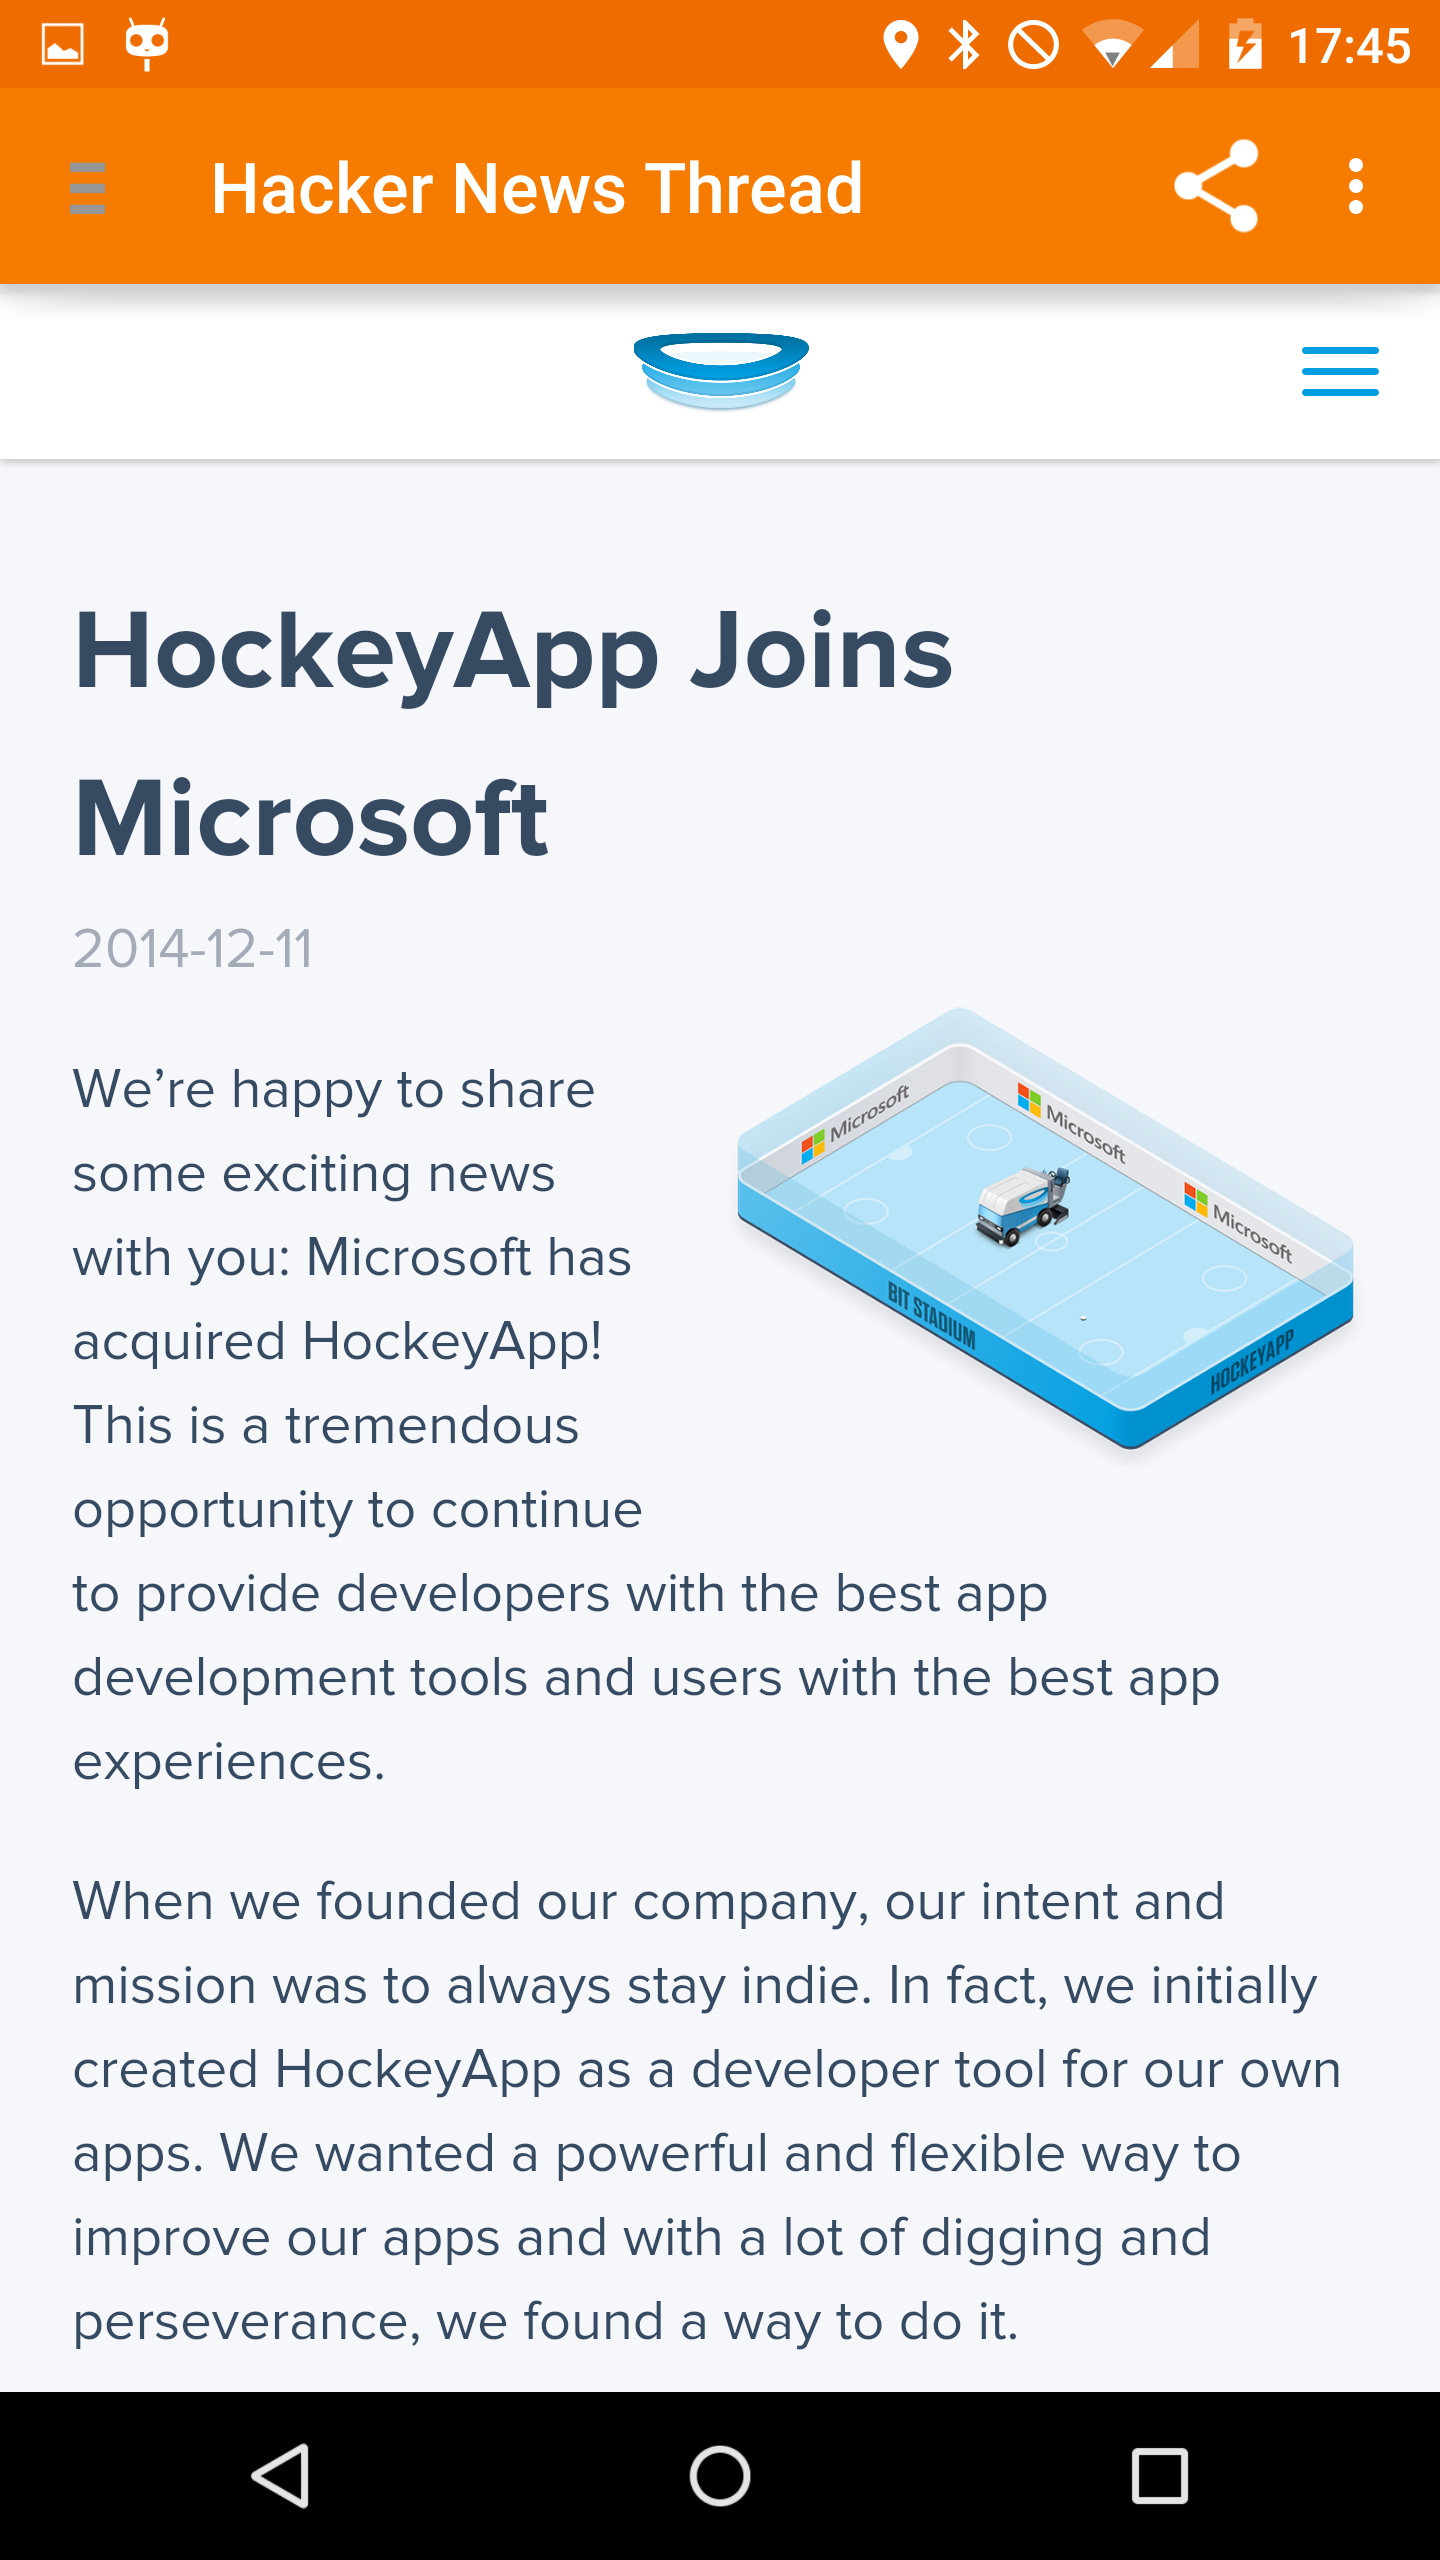
\includegraphics[width=0.3\textwidth]{webView.png}
\end{center}

The web view gives allows the user to view a story external to Hacker News within our application. When a user taps on a story they will be provided this view in order to read the article they have selected. In addition to the standard web view within Android this webview also gives functionality for a user to share their story through another application (Hangouts, Gmail etc.) In addition to this the user can also opt to open the story in their default web browser if they require more functionality.

\subsection*{Settings View}

\begin{center}
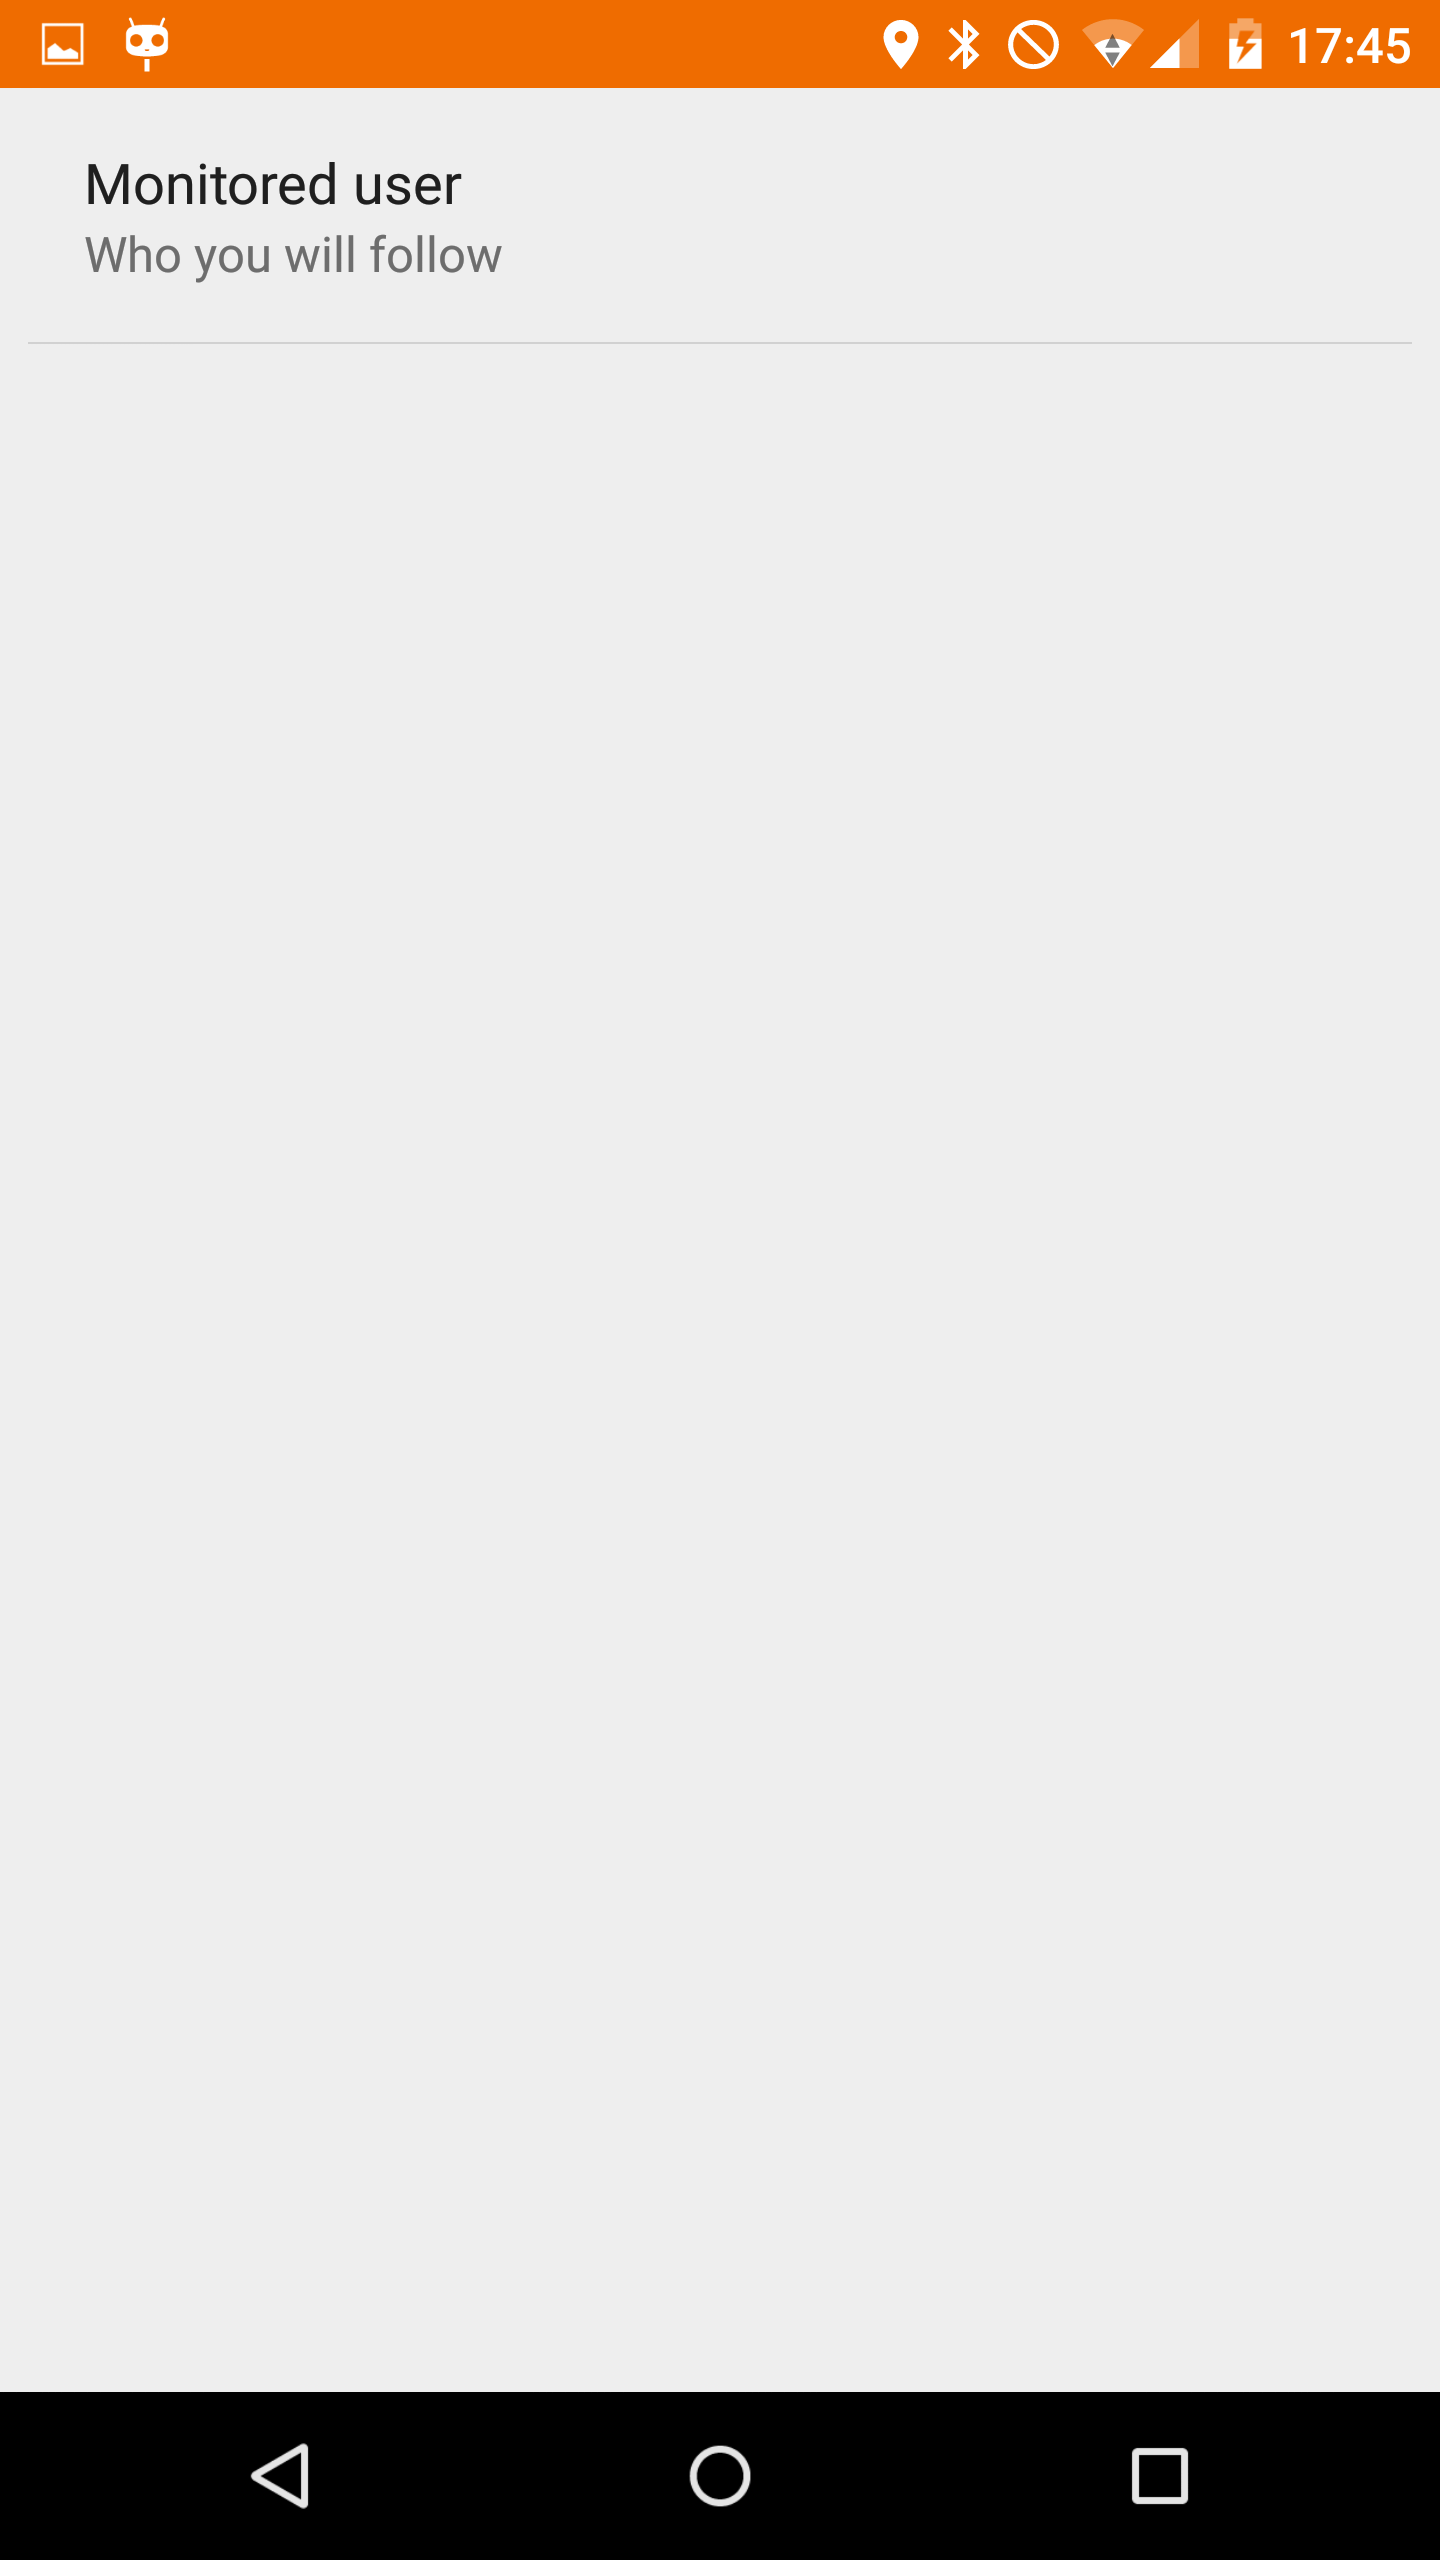
\includegraphics[width=0.3\textwidth]{settings.png}
\end{center}

The Settings view allows a user to change features on the application to suit their needs. For example a user may wish to change the number of stories that are fetched at once...

\section*{Technical Requirements}

\begin{itemize}
	\item{Have a minimum of three distinct screens}
	\begin{itemize}
		\item{The application consists of four distinct screens. These are:}
		\begin{itemize}
			\item{Main View - ‘Top 100 Stories'}
			\item{Comments View for a given story}
			\item{Web View}
			\item{Settings View}
		\end{itemize}
		\end{itemize}
		\item{Work properly with the app lifecycle (including rotate screen changes)}
		\begin{itemize}
			\item{On a phone the application can dynamically resize depending on the screen orientation. In addition to this the application can also supports side-by-side viewing on tablets. When viewed in landscape on a tablet the stories will be displayed in a fragment on the left of the screen with either the web view or comments being displayed on the right side. This is shown below:}
			\\
			\begin{center}
				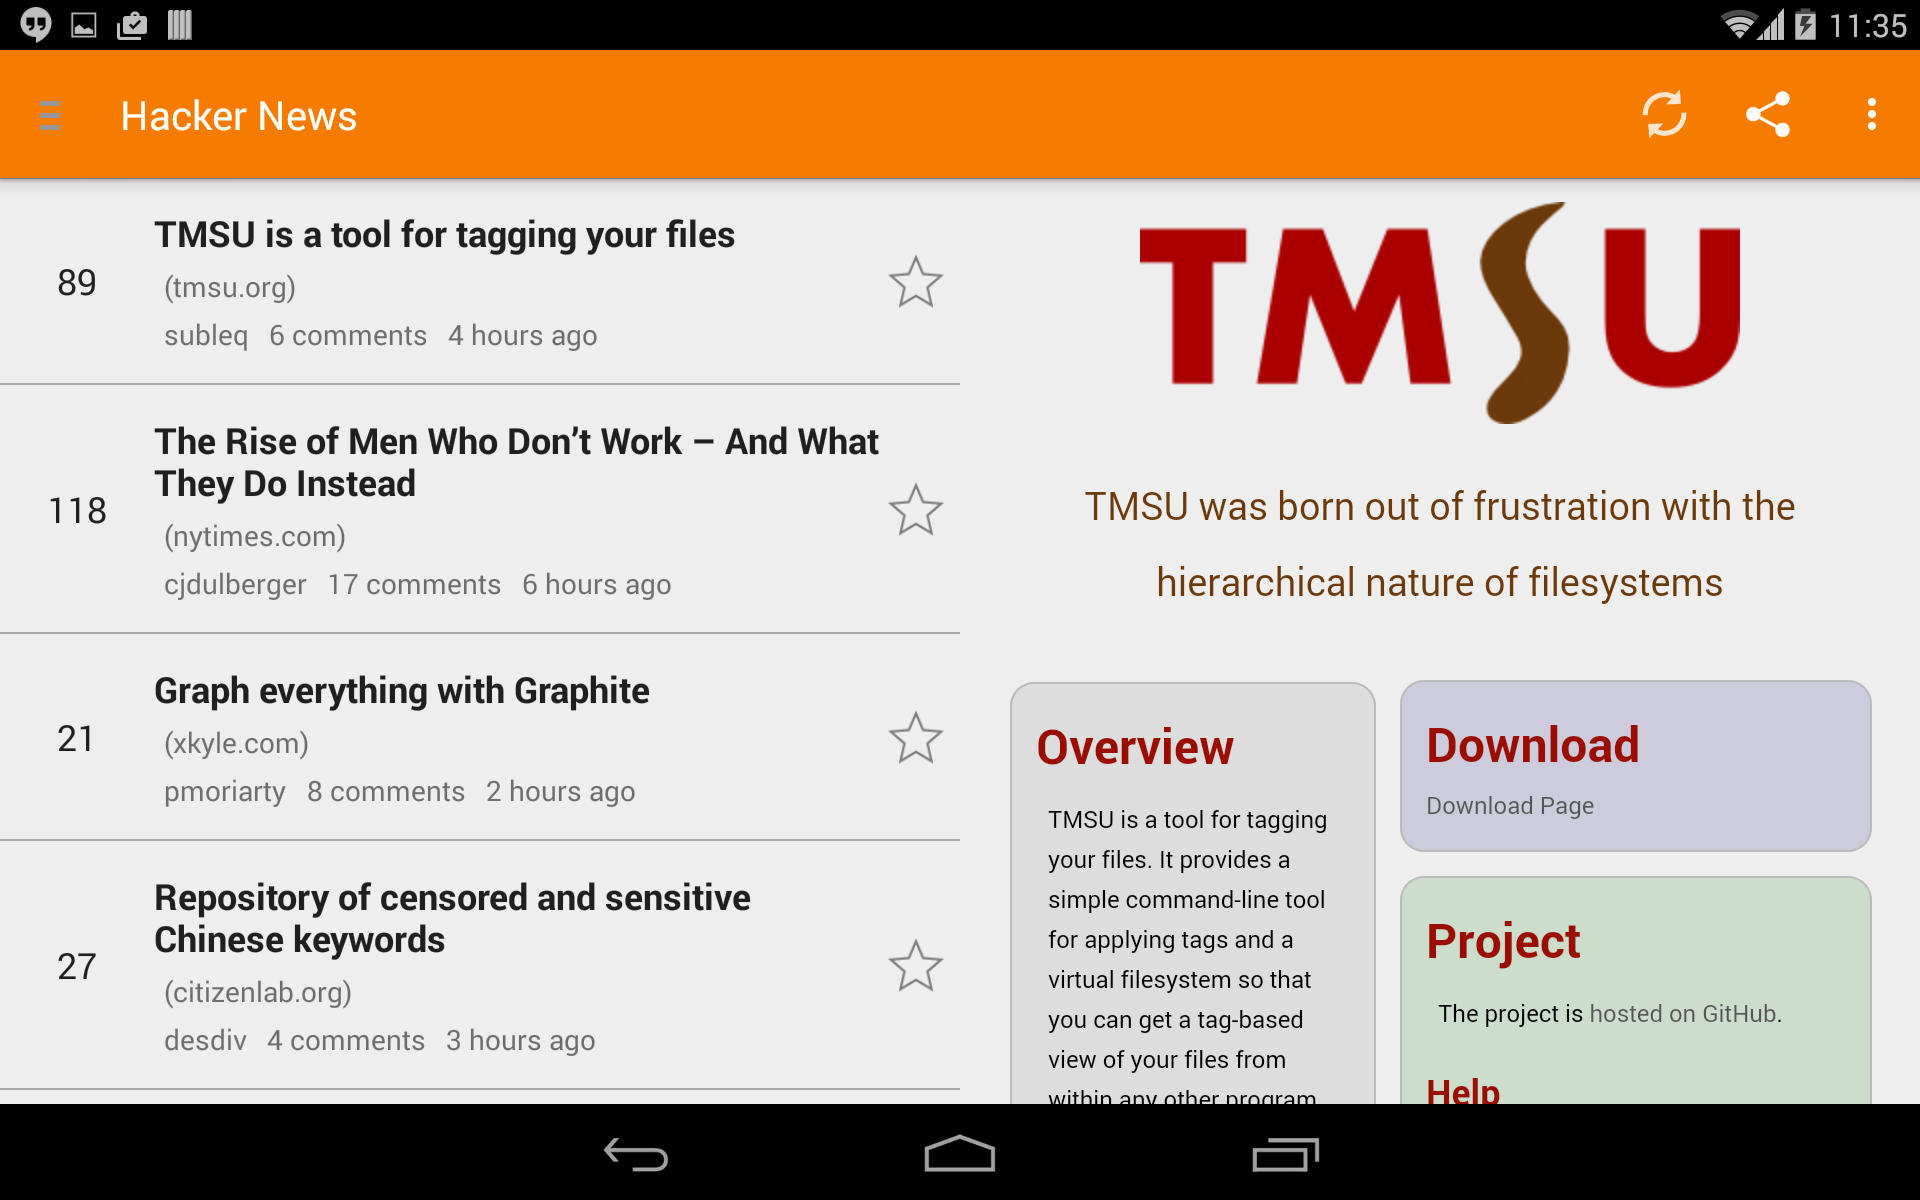
\includegraphics[width=0.3\textwidth]{tabletWeb.png}
				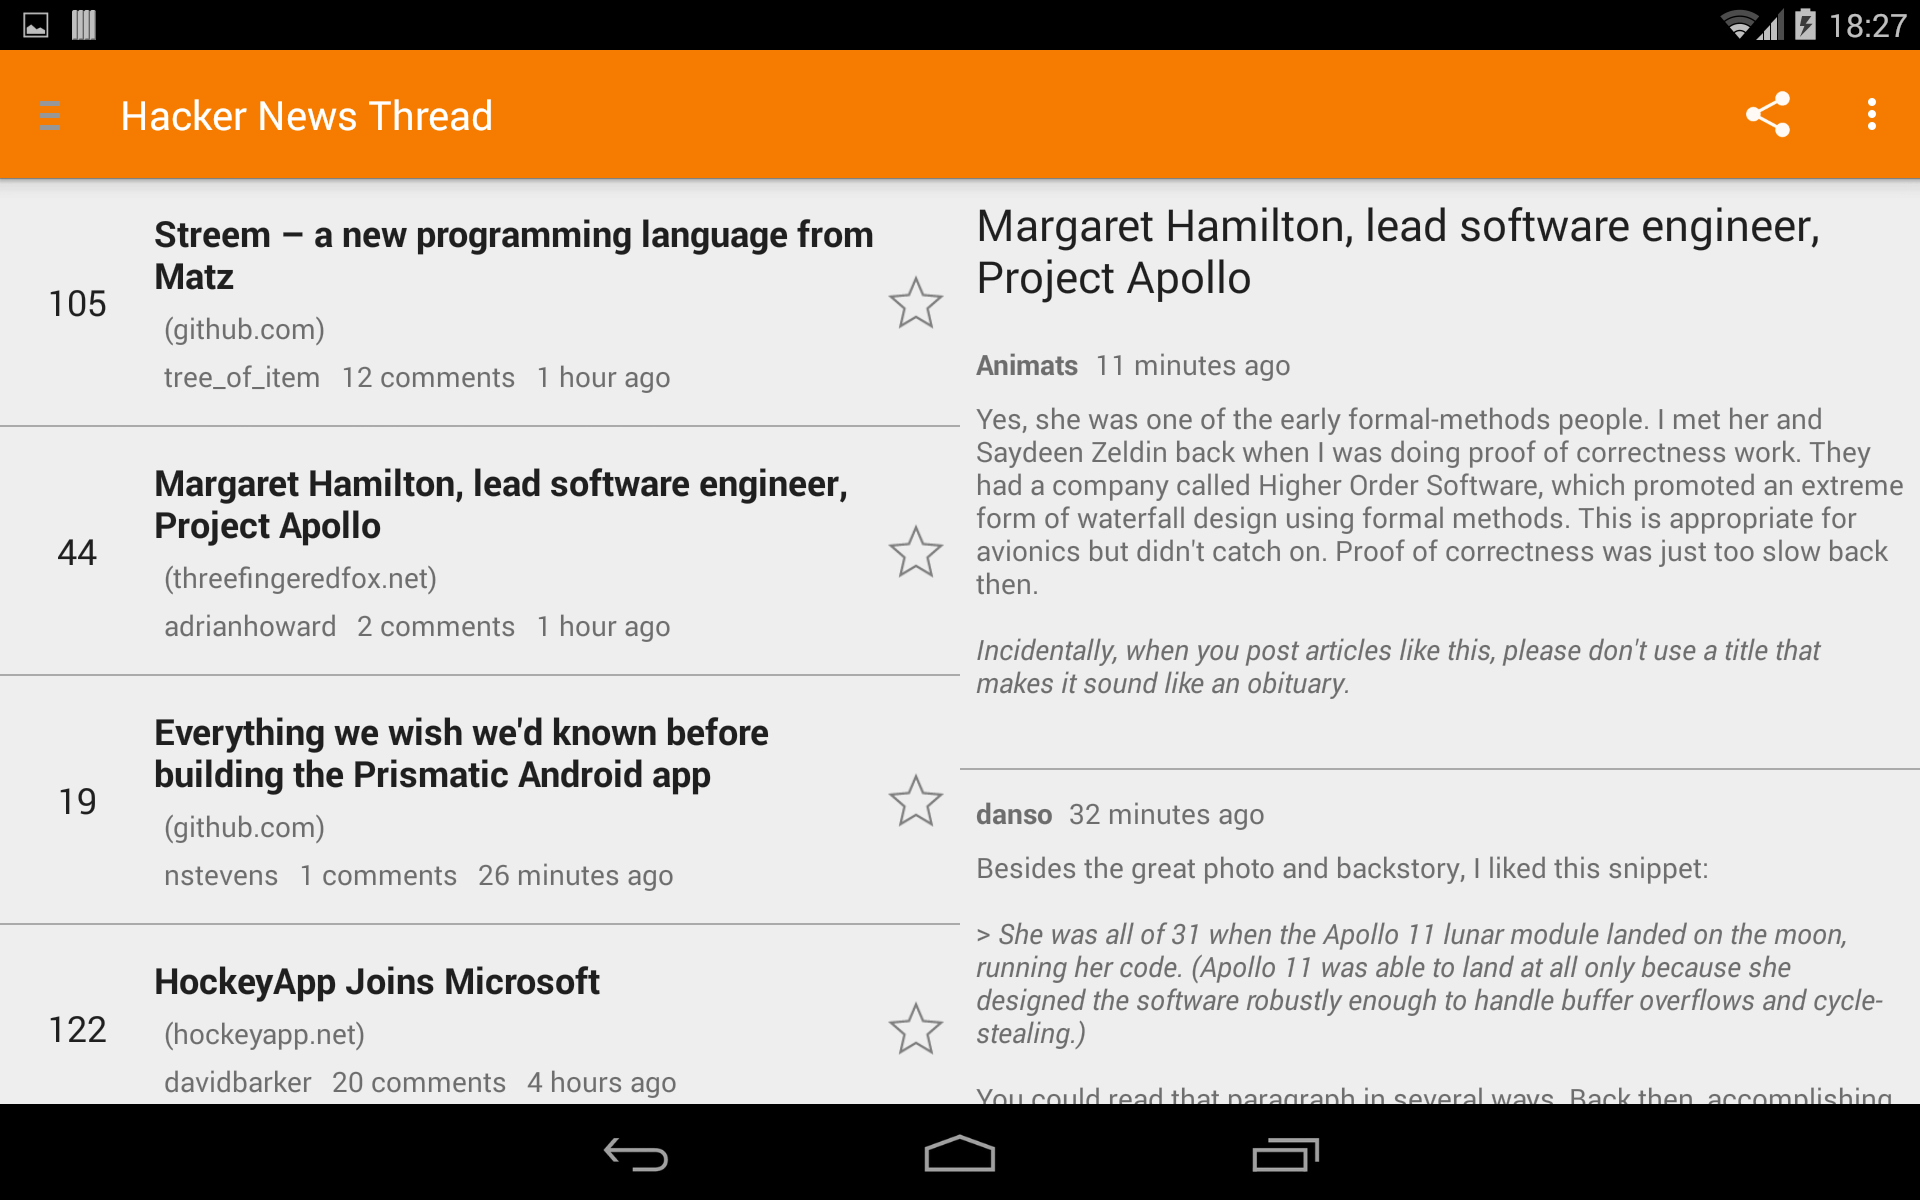
\includegraphics[width=0.3\textwidth]{tabletComments.png}
			\end{center}
	\end{itemize}
	\item{Use permissions and use them responsibly}
	\begin{itemize}
		\item{Our application makes use of network permissions in order to make API requests to Hacker News. We have designed our app with network use in mind in order to minimise the amount of API calls made and the network traffic generated.}
		\item{We have also used local storage permissions in order to save the threads that the user is following along with any external users that they may want to follow.}
		\item{An additional permission we have also added the ‘Receive Boot Completed' permission in order to implement our service. Once our app has been notified that the device has booted it will then start the backend service to manage notifications for updates to followed Users and Threads.}
	\end{itemize}
	\item{Use Intents to move inside your app and to an outside app}
	\begin{itemize}
		\item{Our app uses intents to connect to outside services such as Google Chrome for opening Stories and also sharing applications such as Hangouts or Gmail for the share functionality.}
		\item{Intents are used within the application to handle the interactivity between the Items and Web/Comments View when a tablet is rotated.}
	\end{itemize}
	\item{Create and use your own ContentProvider}
	\begin{itemize}
		\item{The application has the ability to load Hacker News URLs within the application. When opened on a device with our application installed the User can decide to go directly either the comments or web view depending on the type of link accessed. In addition to this, going to the basic URL for Hacker News will open the application with the Top 100 shown.}
	\end{itemize}
	\item{Create and use your own custom Loader}
	\item{The application uses a loader to monitor the database of watched items from the service. This means that when the user favourites an item from the app, and it is added to the database, the service can instantly start monitoring the API endpoint for changes. Because the LoaderManager is usually closely tied to the activity lifecycle that it occupies, our loader is also started and destroyed manually inside the service.}
	\item{Make use of local storage}
	\begin{itemize}
		\item{The application uses local storage to keep a record of Threads and Users that the user has subscribed to.}
	\end{itemize}
\end{itemize}

\section*{Optional Requirements}

\begin{itemize}
	\item{Receive Broadcast events and make use of them in meaningful ways}
	\begin{itemize}
		\item{Our application creates a broadcast on when the device boots in order to start the service for Comments/User updates}
	\end{itemize}
	\item{Create and use a Custom View}
	\begin{itemize}
		\item{The Top 100 Comments pages is a custom view}
	\end{itemize}
	\item{Implement ShareActionProvider}
	\begin{itemize}
		\item{ShareActionProviders are implemented on both the Web View and Comments fragment. This functionality will allow a user to share the URL of the current page they are looking at to applications such as Hangouts or Gmail.}
	\end{itemize}
	\item{Use Services}
	\begin{itemize}
		\item{The application has it's own implementation of a service which connects to Firebase and listens to the Hacker News service. Firebase then informs the service of new content added to watched Threads/Users and generates a notification on the device.}
	\end{itemize}
	\item{Use Notifications}
	\begin{itemize}
		\item{Notifications are generated when our service discovers updates to watched Threads or Users.}
	\end{itemize}
	\item{Capture touch gestures and make reasonable use of them}
	\begin{itemize}
		\item{When used in landscape bot on phones and tablets swiping left or right can flip between the Webview or Comments fragments}
	\end{itemize}
\end{itemize}
\pagebreak
\section*{Test Plans}

Our test plans have been designed on a per-view basis. From each view there are certain expected behaviours which have been implemented, we have used the expected behavior as a basis for our tests.

\subsection*{Top 100 View}

\begin{center}
    \begin{tabular}{ | p{5cm} | p{5cm} | p{5cm} |}
    \hline
    \textbf{Action} & \textbf{Expected Behaviour} & \textbf{Actual Behaviour} \\
    \hline
    Top 100 stories displayed on Application are a mirror of the current Top 100 on the Hacker News website & Stories will match exactly at any given time & As expected   \\ 	\hline
    Scroll down on Top 100 & Stories will be fetched in groups of 10 up until 100 are displayed at once & As expected \\ 
    \hline
    On tap of a Story title & A webview is displayed for the URL associated with that story & As expected \\
    \hline
	On tap of \# Comments & A comments view is opened for the story selected & As expected \\
	\hline
	On tap of ‘Star' of a Story & Star turns opaque & As expected \\ & User subscribes to this Story. & \\ & User receives push notifications on any new comments for the subscribed thread & \\
	\hline
	On tap of Refresh icon in action bar & Stories are Refreshed & As expected \\
	\hline
	On tap of ‘Burger Menu' & Side Menu is displayed & As expected \\
	\hline
    \end{tabular}
\end{center}

\subsection*{Web View}

\begin{center}
\begin{tabular}{ | p{5cm} | p{5cm} | p{5cm} |}
	\hline
	\textbf{Action} & \textbf{Expected Behaviour} & \textbf{Actual Behaviour} \\
    \hline
	On load of Web View & Correct URL is loaded and displayed & As expected \\
	\hline
	Scrolling on web view & Full page is displayed & As expected \\
	\hline
	Swipe left on View & App returns to the main View & As expected \\
	\hline
	Tap of ‘Three Dots' & Open in Browser option shown & As expected \\
	\hline
	Long press of Thread title & Current displayed web view is opened in the devices' default browser & As expected \\
	\hline
	Tap of Share button & Dialog shown for User to decide Share app & As expected \\
	\hline
Tap of a Share app & URL for the current selected story is passed to the app selected. Test case: Hangouts & As expected \\
	\hline
Tap of Default Share app (Displayed once a share app is chosen) & URL for current story is passed to the Default app & As expected \\
	\hline
Swipe left on Webview & App returns to Story View with location saved & As expected \\
	\hline

\end{tabular}
\end{center}

\subsection*{Comments View}

\begin{center}
\begin{tabular}{ | p{5cm} | p{5cm} | p{5cm} |}
	\hline
	\textbf{Action} & \textbf{Expected Behaviour} & \textbf{Actual Behaviour} \\
	\hline
	On load of Comments View & Correct comments for the chosen story are displayed & As expected \\
	\hline
	On load of Comments View & All first-level comments for the chosen story are displayed & As expected \\
	\hline
	Tap of 'Show More' button & The next level of comments (replies) are displayed for the comment in question & As expected \\
	\hline
	Swipe left on Comments View & App returns to the main View with location on Stories saved & As expected \\
	\hline
	Tap of Refresh button & Comments are force refreshed & As expected \\
	\hline
	Tap of Share button & Dialog shown for User to decide Share app & As expected \\
	\hline
	Tap of a Share app & URL for the current selected story is passed to the app selected. Test case: Hangouts & As expected \\
	\hline
	Tap of Default Share app (Displayed once a share app is chosen) & URL for current story is passed to the Default app & As expected \\
	\hline
\end{tabular}
\end{center}

\subsection*{Sidebar Menu}
\begin{center}
\begin{tabular}{ | p{5cm} | p{5cm} | p{5cm} |}
	\hline
	\textbf{Action} & \textbf{Expected Behaviour} & \textbf{Actual Behaviour} \\
	\hline
	Tap of ‘Burger' menu & Sidebar is expanded & As expected \\
	\hline
	Tap of Top Stories option & Top Stories fragment is loaded & As expected \\
	\hline
	Tap of Users option & View for users followed is loaded & As expected \\
	\hline
	Tap of Subscribed Threads option & View for subscribed threads loaded & As expected \\
	\hline
	Tap of Settings option & Settings fragment is loaded & As expected \\
	\hline
\end{tabular}
\end{center}

\subsection*{Settings View}
\begin{center}
\begin{tabular}{ | p{5cm} | p{5cm} | p{5cm} |}
	\hline
	\textbf{Action} & \textbf{Expected Behaviour} & \textbf{Actual Behaviour} \\
	\hline	
	On tap of ‘Users' section & Dialog opened for App user to follow Hacker News Users & As expected \\
	\hline
	On adding a User to follow & Adding a User will add them to ‘Added Users' list & As expected \\ & Notifications will be generated for any submissions by this User & \\
	\hline
	On tap of 'Number of stories to load' & Dialog shown to allow user to select stories to load & As expected \\
	\hline
	On choosing the number of stories to display & Option saved and remembered. Number of stories chosen are fetched in one load & As expected \\
	\hline
\end{tabular}
\end{center}

\section*{Issues and Difficulties Encountered}

\subsection*{Front-end}

From the initial designs of our application we always intended to have two different main screens, a list of links and a webview/comments screen. Where the screen had a larger enough width, i.e a tablet, both of these screens would be displayed next to each other simultaneously.
\\
\\
When it came to implementing this, for simplicity xml layout files were preferred over programmatic ones. The initial idea was to have one activity per screen, but use two layouts to change the list of links screen based on device width. The wider screen layout would display the content of the second webview/comment screen on the right hand side.
\\
\\
However, this design caused an issue when rotating the link screen on a wide device. In landscape the user may be in the middle of viewing a page/comments alongside the story list but on switching to portrait mode, the page/comments would be hidden and only a list of stories displayed. A more correct behaviour would be to show only the webpage/comments in portrait mode if the user was viewing the a particular story. To solve this problem the behaviour of split-screen activities had to be rethought. Rather than having the stories page change its layout on rotation, now the webview or comments page change instead.
\\
\\
In addition to fixing the behaviour detailed above, this also had the benefit of making it easier handle opening of the app externally. Opening the link https://news.ycombinator.com/ now allows you to open a URL in our application, showing the user the list of stories activity, where as appending /item?id=XXXX takes you to the webview/comments activity. 
\\
\\
The largest potential drawback to this approach was duplication of effort for the list of links fragment's activity callbacks. To avoid this, we changed both activities to inherit from a base class implementing shared callbacks. In the end though this probably introduced unwanted complexity as most non-trivial callbacks were different for both activities.

\subsection*{Back-end}

Our connection to Hacker News is dependent on their API which is provided through Firebase. Firebase is a widely used provider of real-time information so when designing this app we expected the backend to have a well-defined structure. Unfortunately the API implemented by Hacker News is relatively new in design, and as such has some issues. When designing an application for mobile devices we took into consideration the additional load on already limited resources - including the network, battery and CPU usage. Because of this we designed our application to minimise the API requests in order to create a functional application that does not tax on the devices resources.
\\
\\
One of the first issues we encountered was the layout of the data returned in an API call. We found that all returned information was of type Item. Many of these Items shared the same parameters but did not enforce the use of every field in the object. This created issues on our back-end when trying to pass values throughout the system as null values or parameters that are non-existent would appear on the front-end - this created crashes in the application. We also found these issues would appear infrequently due to the fact that different Threads could appear at different times due to the current state of the Top 100. On particular time we found that the Top 100 would not load a Job post as the object returned was missing a comments field entirely. This was not documented in the API and meant we then needed to provide a check on the application side to create a new class for Job posts and handle the lack of comment value.
\\
\\
A second issue on the API was the Top 100 request itself. We found that the default API request returned a list of 100 Ids for the Threads required. Because of this we needed to redesign the Threads View to not show the top 100 by default, but to instead display the full amount required in an interval defined by the application. We found that increments of 10 would fill around a two full screens worth of threads and allow a user to scroll whilst a call was made for the next increment of 10. This would continue until 100 Threads were displayed in the view. We decided to implement this behaviour due to the amount of API calls required it the fetch of on Thread. First the application makes an API call for the Top 100 stories, this returns the list of IDs for these stories, we then stored these ready for use in any further API calls. To request the first 10 Threads we then use the list we stored to find the ID of each Thread, at this point we make an API request to get the details of each Thread by searching for it's ID, the returned information is then put into a class and passed to the front-end for display. We found that this implementation considerably brought down the resources required by the application but still enabled the next 10 Threads to be fetched and displayed without too much delay to the User.
\\
\\
One piece of functionality we were also intending to add was the ability to filter the displayed Threads by their type. Our first design included using a call to the API to request new content, however this was not implemented in the way it was expected. An API request could be made request the MaxID on Hacker News - thus giving us the ID of the newest item on Hacker News itself. From this point, the only way to find the items required would be to decrement the ID value and request the second newest item, continuing until we have the number of items we are looking for. Each item would require it's own API call to check whether it was a Story, Job, AskHN, Poll or Comment. This would required potentially thousands of API requests until a usable number of items were found for the User to view. Again, when considering the load this would add to the device this would not be desirable.
\\
\\
A second method of implementing filtering would be to use the Top 100 for this, first requesting all 100 items and checking each individual item in order to find whether it is of the desired type and discarding any items that do not match. We found that while this method of implementation would require less load, the result it would yield would make it impractical. This is due to the fact that at any given point 95\% of the items on the Top 100 were Stories. Filtering on anything other than this would usually display a single item of the desired type, this was not a very useful feature to implement.
\\
\\
In addition to adding filtering the above issues also prevented us from being able to show the newest stories. This is due to the fact that when we receive the current highest ID this includes every item id in the Hacker News website. In particular we found that these IDs were tended to below to comments on a thread, however without requesting the object by it's ID we were not able to be sure what the object was. To be able to find the one hundred newest Threads we would be required to make around five hundred requests to the API, check each individual object returned to see if it was of type Thread (no Comment or Poll Option) and then discard any stories not required. This implementation would have added considerable strain to a device both in terms of network usage and also the time required to process the information.

\end{document}
